%% ============================================================
%%  Topological Classification via Parametric Manifolds
%%  Presentación Académica Completa — Beamer / LaTeX
%%  Autor: Hugo Campos Castro
%% ============================================================

\documentclass[aspectratio=169,10pt]{beamer}

% ── Tema ──────────────────────────────────────────────────────
\usetheme{Madrid}
\usecolortheme{default}

% ── Paleta de colores personalizada ───────────────────────────
\definecolor{primary}{HTML}{0D1B2A}      % Azul marino profundo
\definecolor{accent}{HTML}{00C8FF}       % Celeste eléctrico
\definecolor{accent2}{HTML}{FF3366}      % Rosa eléctrico (SHM)
\definecolor{accent3}{HTML}{00E676}      % Verde
\definecolor{bg}{HTML}{F7F9FC}           % Fondo claro
\definecolor{darkgray}{HTML}{2D3748}
\definecolor{medgray}{HTML}{718096}

\setbeamercolor{frametitle}{bg=primary, fg=white}
\setbeamercolor{title}{fg=white}
\setbeamercolor{subtitle}{fg=accent}
\setbeamercolor{author}{fg=accent}
\setbeamercolor{date}{fg=white}
\setbeamercolor{block title}{bg=primary, fg=accent}
\setbeamercolor{block body}{bg=bg, fg=darkgray}
\setbeamercolor{block title alerted}{bg=accent2!80, fg=white}
\setbeamercolor{block body alerted}{bg=accent2!10, fg=darkgray}
\setbeamercolor{block title example}{bg=accent3!70!black, fg=white}
\setbeamercolor{block body example}{bg=accent3!10, fg=darkgray}
\setbeamercolor{palette primary}{bg=primary, fg=white}
\setbeamercolor{palette secondary}{bg=primary!80, fg=white}
\setbeamercolor{palette tertiary}{bg=primary!60, fg=white}
\setbeamercolor{palette quaternary}{bg=primary!40, fg=white}
\setbeamercolor{structure}{fg=primary}
\setbeamercolor{section in toc}{fg=primary}
\setbeamercolor{itemize item}{fg=accent}
\setbeamercolor{itemize subitem}{fg=accent2}
\setbeamercolor{itemize subsubitem}{fg=accent3}

% ── Fuente ────────────────────────────────────────────────────
\usepackage[T1]{fontenc}
\usepackage[utf8]{inputenc}
\usepackage{lmodern}

% ── Paquetes ──────────────────────────────────────────────────
\usepackage[spanish]{babel}
\usepackage{amsmath,amssymb,amsfonts}
\usepackage{graphicx}
\usepackage{booktabs}
\usepackage{xcolor}
\usepackage{tikz}
\usepackage{tcolorbox}
\usetikzlibrary{arrows.meta, positioning, shapes.geometric, backgrounds, decorations.pathreplacing}
\tcbuselibrary{breakable}

% ── Comandos útiles ───────────────────────────────────────────
\newcommand{\highlight}[1]{\textcolor{accent}{\textbf{#1}}}
\newcommand{\hl}[1]{\colorbox{accent!20}{\strut#1}}
\newcommand{\pval}[1]{\textcolor{accent2}{\textbf{#1}}}

% ── Box de definición ─────────────────────────────────────────
\tcbset{
  mydef/.style={
    sharp corners, boxrule=1pt,
    colback=primary!5, colframe=accent, coltitle=white,
    fonttitle=\bfseries\small, title={#1},
  },
  myex/.style={
    sharp corners, boxrule=1pt,
    colback=accent3!8, colframe=accent3!60!black, coltitle=white,
    fonttitle=\bfseries\small, title={#1},
  },
  mywarn/.style={
    sharp corners, boxrule=1pt,
    colback=accent2!10, colframe=accent2, coltitle=white,
    fonttitle=\bfseries\small, title={#1},
  },
}

% ── Metadata ──────────────────────────────────────────────────
\title[Clasificación Topológica Paramétrica]{%
  Topological Classification via\\Parametric Manifolds}
\subtitle{FM $\to$ AM $\to$ GAM $\to$ SHM \ $\|$ \ NSGA-II $\to$ MGDA}
\author[H. Campos]{Hugo Campos Castro}
\date{\today}
\institute{Departamento de Ciencias de la Computación}

% ── Configuración de bloques ──────────────────────────────────
\setbeamertemplate{blocks}[rounded][shadow=false]
\setbeamertemplate{navigation symbols}{}
\setbeamertemplate{footline}[frame number]

%% ============================================================
\begin{document}

%% ── PORTADA ─────────────────────────────────────────────────
{
\setbeamercolor{background canvas}{bg=primary}
\begin{frame}[plain]
  \vspace{1.5cm}
  \centering
  {\Huge\bfseries\textcolor{white}{Clasificación Topológica}\\[4pt]}
  {\Huge\bfseries\textcolor{accent}{via Variedades Paramétricas}\\[12pt]}
  {\large\textcolor{white!70}{FM $\;\longrightarrow\;$ AM $\;\longrightarrow\;$ GAM $\;\longrightarrow\;$ SHM}}\\[4pt]
  {\large\textcolor{white!70}{NSGA-II $\;\longrightarrow\;$ MGDA}}\\[20pt]
  \rule{8cm}{0.4pt}\\[10pt]
  {\normalsize\textcolor{white}{Hugo Campos Castro}\\[4pt]}
  {\small\textcolor{white!60}{\today}}
\end{frame}
}

%% ── TABLA DE CONTENIDOS ─────────────────────────────────────
\begin{frame}{Contenido de la Presentación}
  \tableofcontents
\end{frame}

%% ============================================================
\section{Motivación y Contexto}
%% ============================================================

\begin{frame}{El Problema: Clasificación No Lineal}
  \begin{columns}[T]
    \begin{column}{0.5\textwidth}
      \begin{block}{¿Qué buscamos?}
        Separar clases en espacios donde \textbf{ningún hiperplano} puede hacer el trabajo.
      \end{block}
      \vspace{6pt}
      \textbf{Enfoques clásicos:}
      \begin{itemize}
        \item \textbf{SVM + kernel trick}: deforma el espacio, pierde interpretabilidad.
        \item \textbf{Redes Neuronales}: millones de parámetros, total caja negra.
        \item \textbf{Árboles}: solo cortes ortogonales — no curvas suaves.
      \end{itemize}
      \vspace{6pt}
      \begin{alertblock}{Limitación crítica}
        Todos los métodos clásicos sacrifican \textbf{interpretabilidad} por potencia.
      \end{alertblock}
    \end{column}
    \begin{column}{0.48\textwidth}
      \begin{tcolorbox}[mydef={Nuestra propuesta}]
        Construimos un \textbf{colector paramétrico cerrado} $M \subset \mathbb{R}^D$ que se \emph{pliega} para \textbf{encapsular} la clase objetivo en su topología nativa.\\[6pt]
        $\Rightarrow$ La ecuación de la frontera es \textbf{explícita y extraíble}.\\[4pt]
        $\Rightarrow$ \highlight{White-Box}: total interpretabilidad analítica.
      \end{tcolorbox}
    \end{column}
  \end{columns}
\end{frame}

\begin{frame}{El Viaje Evolutivo: 5 Generaciones}
  \centering
  \begin{tikzpicture}[
    box/.style={draw, rounded corners, fill=primary!10, text width=2.4cm, align=center, font=\footnotesize\bfseries, minimum height=1cm},
    arr/.style={-Stealth, thick, color=accent},
    node distance=0.5cm,
  ]
  \node[box, fill=primary!20] (fm)  {Gen.\ 1\\FM-NSGA-II\\{\tiny Fourier}};
  \node[box, right=0.5cm of fm]     (am)  {Gen.\ 2\\AM-NSGA-II\\{\tiny Chebyshev}};
  \node[box, right=0.5cm of am]     (gam) {Gen.\ 3\\GAM-NSGA-II\\{\tiny Aditivo}};
  \node[box, right=0.5cm of gam, fill=accent2!20]  (shm) {Gen.\ 4\\SHM-NSGA-II\\{\tiny Arm.\ Esf.}};
  \node[box, right=0.5cm of shm, fill=accent3!20]  (mgda){Gen.\ 5\\MGDA\\{\tiny Gradientes}};
  \draw[arr] (fm)  -- (am);
  \draw[arr] (am)  -- (gam);
  \draw[arr] (gam) -- (shm);
  \draw[arr] (shm) -- (mgda);
  \node[below=0.25cm of fm,  font=\tiny, text=medgray]  {Alta expresividad};
  \node[below=0.25cm of am,  font=\tiny, text=medgray]  {$O(D\!+\!H)$, sin $t^*$};
  \node[below=0.25cm of gam, font=\tiny, text=medgray]  {Auditabilidad axial};
  \node[below=0.25cm of shm, font=\tiny, text=medgray]  {Base 3D};
  \node[below=0.25cm of mgda,font=\tiny\bfseries, text=accent3!70!black] {$>100\times$ veloz};
  \end{tikzpicture}

  \vspace{8pt}
  \begin{columns}[T]
    \begin{column}{0.48\textwidth}
      \textbf{Problema central original:}\\
      FM usa $\sin/\cos$ — no diferenciable globalmente para un error discreto $\Rightarrow$ requería optimizador evolutivo (\textbf{NSGA-II}).
    \end{column}
    \begin{column}{0.48\textwidth}
      \textbf{Hallazgo crítico (Gen. 5):}\\
      AM y GAM \textit{sí} son diferenciables analíticamente $\Rightarrow$ reemplazamos la selección natural por \textbf{gradientes exactos (MGDA)}.
    \end{column}
  \end{columns}
\end{frame}

%% ============================================================
\section{Formulación Matemática: Los Kernels}
%% ============================================================

\begin{frame}{Concepto Base: El Colector y la Distancia con Signo}
  \begin{columns}[T]
    \begin{column}{0.55\textwidth}
      \begin{tcolorbox}[mydef={Distancia Radial con Signo $D_S$}]
        Para un punto $\mathbf{x}$ y un colector $M$ con centroide $\mathbf{c}$:
        \[
          D_S(\mathbf{x}, M) = d_w(\mathbf{x},\mathbf{c}) - d_w(\mathbf{f}(t^*),\mathbf{c})
        \]
        donde $d_w$ es la distancia euclidiana \textbf{ponderada} y $t^*$ el punto más cercano en la curva.
      \end{tcolorbox}
      \vspace{6pt}
      \textbf{Regla de decisión:}\\
      \begin{itemize}
        \item $D_S < 0$ $\Rightarrow$ \textcolor{accent3}{punto \textbf{dentro}} del colector $\Rightarrow$ clase $+1$
        \item $D_S > 0$ $\Rightarrow$ \textcolor{accent2}{punto \textbf{fuera}} del colector $\Rightarrow$ clase $-1$
      \end{itemize}
    \end{column}
    \begin{column}{0.42\textwidth}
      \begin{tcolorbox}[myex={Ejemplo intuitivo: 2D}]
        {\footnotesize
        Imagina un círculo alrededor de la clase ``\textit{Benigno}''.\\[4pt]
        Un nuevo paciente $\mathbf{x}$:
        \begin{itemize}
          \item Distancia al centro: $4.2$
          \item Radio del colector en esa dirección: $5.0$
          \item $D_S = 4.2 - 5.0 = -0.8 < 0$
        \end{itemize}
        $\Rightarrow$ El paciente está \textbf{dentro} → \texttt{Benigno}.}
      \end{tcolorbox}
    \end{column}
  \end{columns}
\end{frame}

%% ── GEN 1: FM ────────────────────────────────────────────────
\begin{frame}{Generación 1: Fourier Manifold (FM)}
  \begin{columns}[T]
    \begin{column}{0.55\textwidth}
      La curva de frontera se parametriza con \textbf{Series de Fourier}:
      \begin{equation}
        f_d(t) = a_{0,d} + \sum_{k=1}^{H} \bigl( a_{k,d}\cos(kt) + b_{k,d}\sin(kt) \bigr)
      \end{equation}
      \begin{itemize}
        \item $t \in [0, 2\pi)$: parámetro angular.
        \item $H$: armónicos — controla la complejidad oscilatoria.
        \item $d$: índice de dimensión en $\mathbb{R}^D$.
      \end{itemize}
      \begin{alertblock}{Intuyendo $H$}
        \begin{itemize}
          \item $H=0$: punto fijo (sin curva)
          \item $H=1$: \textbf{círculo / elipse} perfecta
          \item $H=3$: "abollar" el círculo — luna, herradura, espiral
        \end{itemize}
      \end{alertblock}
    \end{column}
    \begin{column}{0.42\textwidth}
      \begin{tcolorbox}[mywarn={Limitación}]
        {\footnotesize Evaluar $t^* = \arg\min_t d_w(\mathbf{x}, \mathbf{f}(t))$ requiere búsqueda iterativa.\\[4pt]
        Calcular $\sin/\cos$ es costoso para Big Data.\\[4pt]
        \textbf{No es diferenciable} globalmente respecto al error discreto $\Rightarrow$ obligó a usar \textbf{NSGA-II}.}
      \end{tcolorbox}
      \vspace{6pt}
      {\small\textbf{Cromosoma FM:}\\contiene los coeficientes $\{a_{k,d}, b_{k,d}\}$ y los co-pesos $\mathbf{w}$.}
    \end{column}
  \end{columns}
\end{frame}

\begin{frame}{Generación 1: Cromosoma FM — Visualización}
  \centering
  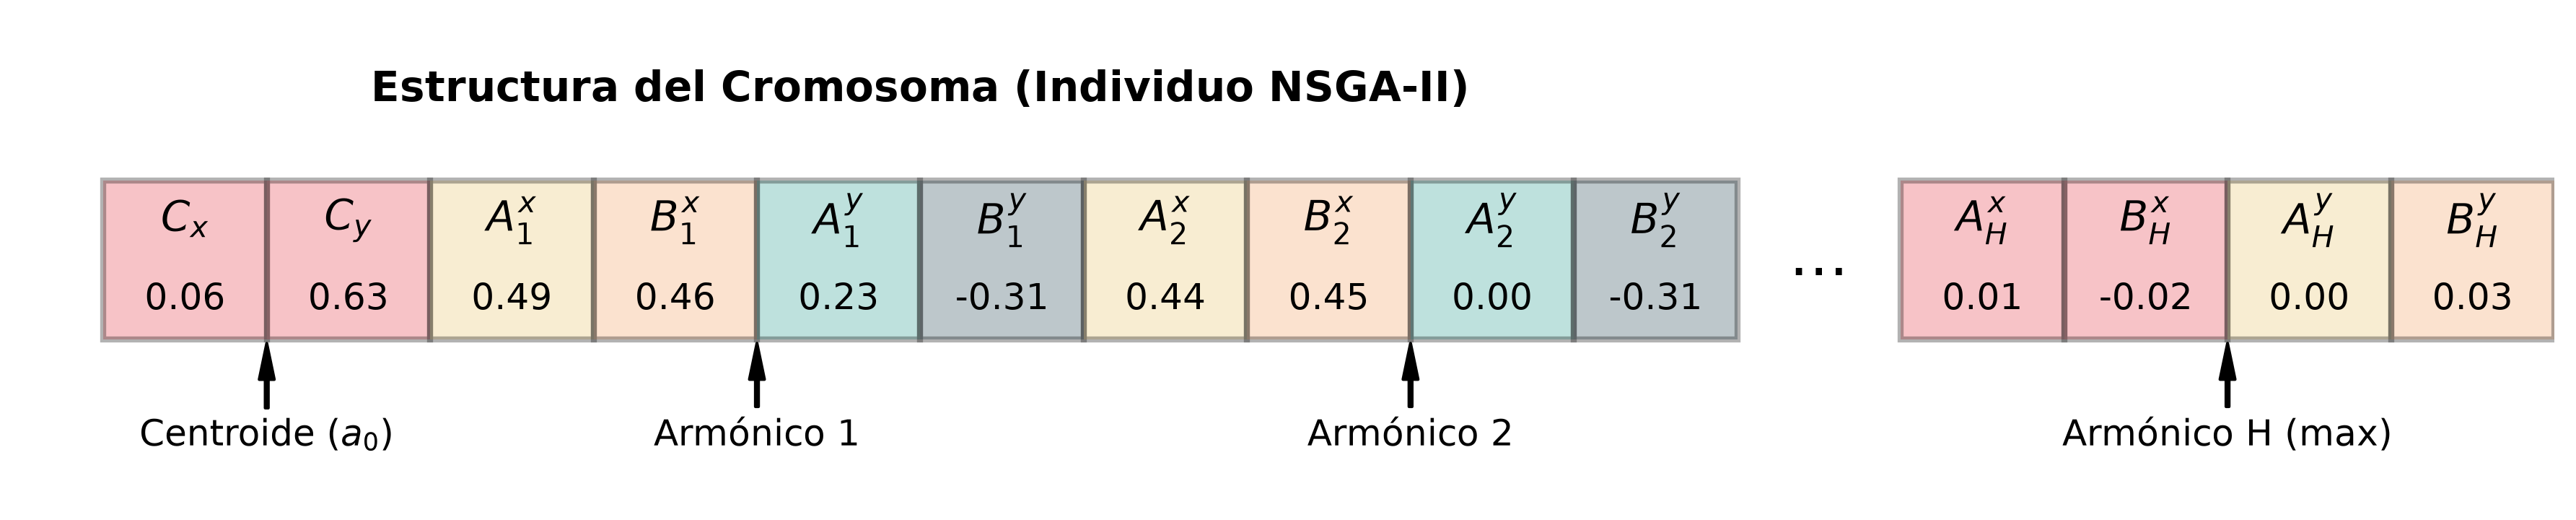
\includegraphics[width=0.85\textwidth]{../build/plot_chromosome.png}
  \vspace{4pt}
  \begin{tcolorbox}[myex={¿Qué vemos?}]
    {\small Los genes (barra de colores) representan los amplitudes $a_{k,d}, b_{k,d}$ por dimensión y armónico. El peso $\mathbf{w}$ (primera sección) actúa como escala por cada feature. Genéticamente, NSGA-II muta estos genes para que la curva resultante englobe la clase objetivo.}
  \end{tcolorbox}
\end{frame}

%% ── GEN 2: AM ────────────────────────────────────────────────
\begin{frame}{Generación 2: Angular Manifold (AM)}
  \textbf{Idea clave:} En vez de parametrizar toda la curva, proyectamos $\mathbf{x}$ sobre un \textbf{eje polar} aprendido $\mathbf{v}$.

  \begin{columns}[T]
    \begin{column}{0.5\textwidth}
      \textbf{Paso 1 — Coseno proyectado:}
      \[
        z = \cos\theta = \frac{\langle \mathbf{x} - \mathbf{c},\, \mathbf{v} \rangle_w}{\|\mathbf{x} - \mathbf{c}\|_w \cdot \|\mathbf{v}\|_w}
      \]

      \textbf{Paso 2 — Radio límite con Chebyshev:}
      \[
        R(\mathbf{x}) = a_0 + \sum_{k=1}^{H} a_k\, T_k(z)
      \]
      Donde $T_k$ son los \textbf{Polinomios de Chebyshev} de primer tipo:
      \[
        T_0=1,\quad T_1=z,\quad T_k = 2z\,T_{k-1} - T_{k-2}
      \]

      \textbf{Paso 3 — Decisión:}
      \[
        D_S = \|\mathbf{x}-\mathbf{c}\|_w - R(\mathbf{x})
      \]
    \end{column}
    \begin{column}{0.47\textwidth}
      \begin{tcolorbox}[myex={Ejemplo médico 30D}]
        {\small El algoritmo descubre el vector ``maestro'' $\mathbf{v}$ en 30D.\\[4pt]
        Para un nuevo paciente $\mathbf{x}$:
        \begin{enumerate}
          \item Computamos $z = \cos(45°) = 0.707$
          \item Evaluamos: $R = a_0 + a_1(0.707) + a_2(2\cdot 0.707^2-1) + ...$
          \item Si $\|\mathbf{x}\|_w = 1.8$ y $R = 2.5$: $D_S = -0.7 < 0 \Rightarrow$ \texttt{clase +1}
        \end{enumerate}
        \textbf{¡Comprimimos 30D a un escalar!}}
      \end{tcolorbox}
      \vspace{4pt}
      \begin{alertblock}{Ganancia}
        Inferencia $\mathcal{O}(D + H)$. \textbf{Sin} búsqueda de $t^*$.
      \end{alertblock}
    \end{column}
  \end{columns}
\end{frame}

\begin{frame}{Generación 2: Cromosoma AM — Visualización}
  \centering
  \includegraphics[width=0.85\textwidth]{../build/plot_angular_chromosome.png}
  \vspace{4pt}
  \begin{tcolorbox}[myex={¿Qué vemos?}]
    {\small El cromosoma AM codifica: el vector $\mathbf{v}$ (eje de proyección), los co-pesos $\mathbf{w}$ y los coeficientes $\{a_k\}$ del polinomio de Chebyshev. NSGA-II evoluciona este cromosoma minimizando el error y la complejidad del borde.}
  \end{tcolorbox}
\end{frame}

%% ── GEN 3: GAM ───────────────────────────────────────────────
\begin{frame}{Generación 3: Generalized Additive Manifold (GAM)}
  \textbf{Idea clave:} Desacoplar las dimensiones — cada eje contribuye \textbf{independientemente} al radio límite.

  \begin{columns}[T]
    \begin{column}{0.55\textwidth}
      El radio límite se consolida aditivamente:
      \[
        R(\mathbf{x}) = a_0 + \sum_{d=1}^{D} w_d \left(\sum_{k=1}^{H} a_{d,k}\, T_k(\hat{x}_d)\right)
      \]
      donde $\hat{x}_d = \frac{x_d - \mu_d}{\sigma_d}$ es la feature estandarizada.

      \vspace{8pt}
      \textbf{Propiedades fundamentales:}
      \begin{itemize}
        \item \highlight{Aditividad} $\Rightarrow$ cada dimensión es separable.
        \item El vector $\mathbf{w} = [w_1, w_2, \ldots, w_D]$ es un índice directo de \textbf{Feature Importance}.
        \item Diferenciable respecto a todos los parámetros $\Rightarrow$ \textbf{habilita MGDA}.
      \end{itemize}
    \end{column}
    \begin{column}{0.42\textwidth}
      \begin{tcolorbox}[myex={Ejemplo: Diagnóstico de Obesidad}]
        {\small Features: $d=1$ Perímetro Abdominal, $d=2$ Color de Ojos.\\[4pt]
        Tras el entrenamiento, el optimizador descubre:
        \[
          w_1 = 0.99,\quad w_2 = 0.001
        \]
        El término $w_2 \cdot (\ldots) \approx 0$.\\[4pt]
        \textbf{Resultado:} El modelo descarta matemáticamente el Color de Ojos sin post-hoc (sin LIME, sin SHAP).}
      \end{tcolorbox}
      \begin{alertblock}{White-Box pura}
        $\mathbf{w}$ es el único certificado de interpretabilidad analítica.
      \end{alertblock}
    \end{column}
  \end{columns}
\end{frame}

\begin{frame}{Generación 3: Cromosoma GAM — Visualización}
  \centering
  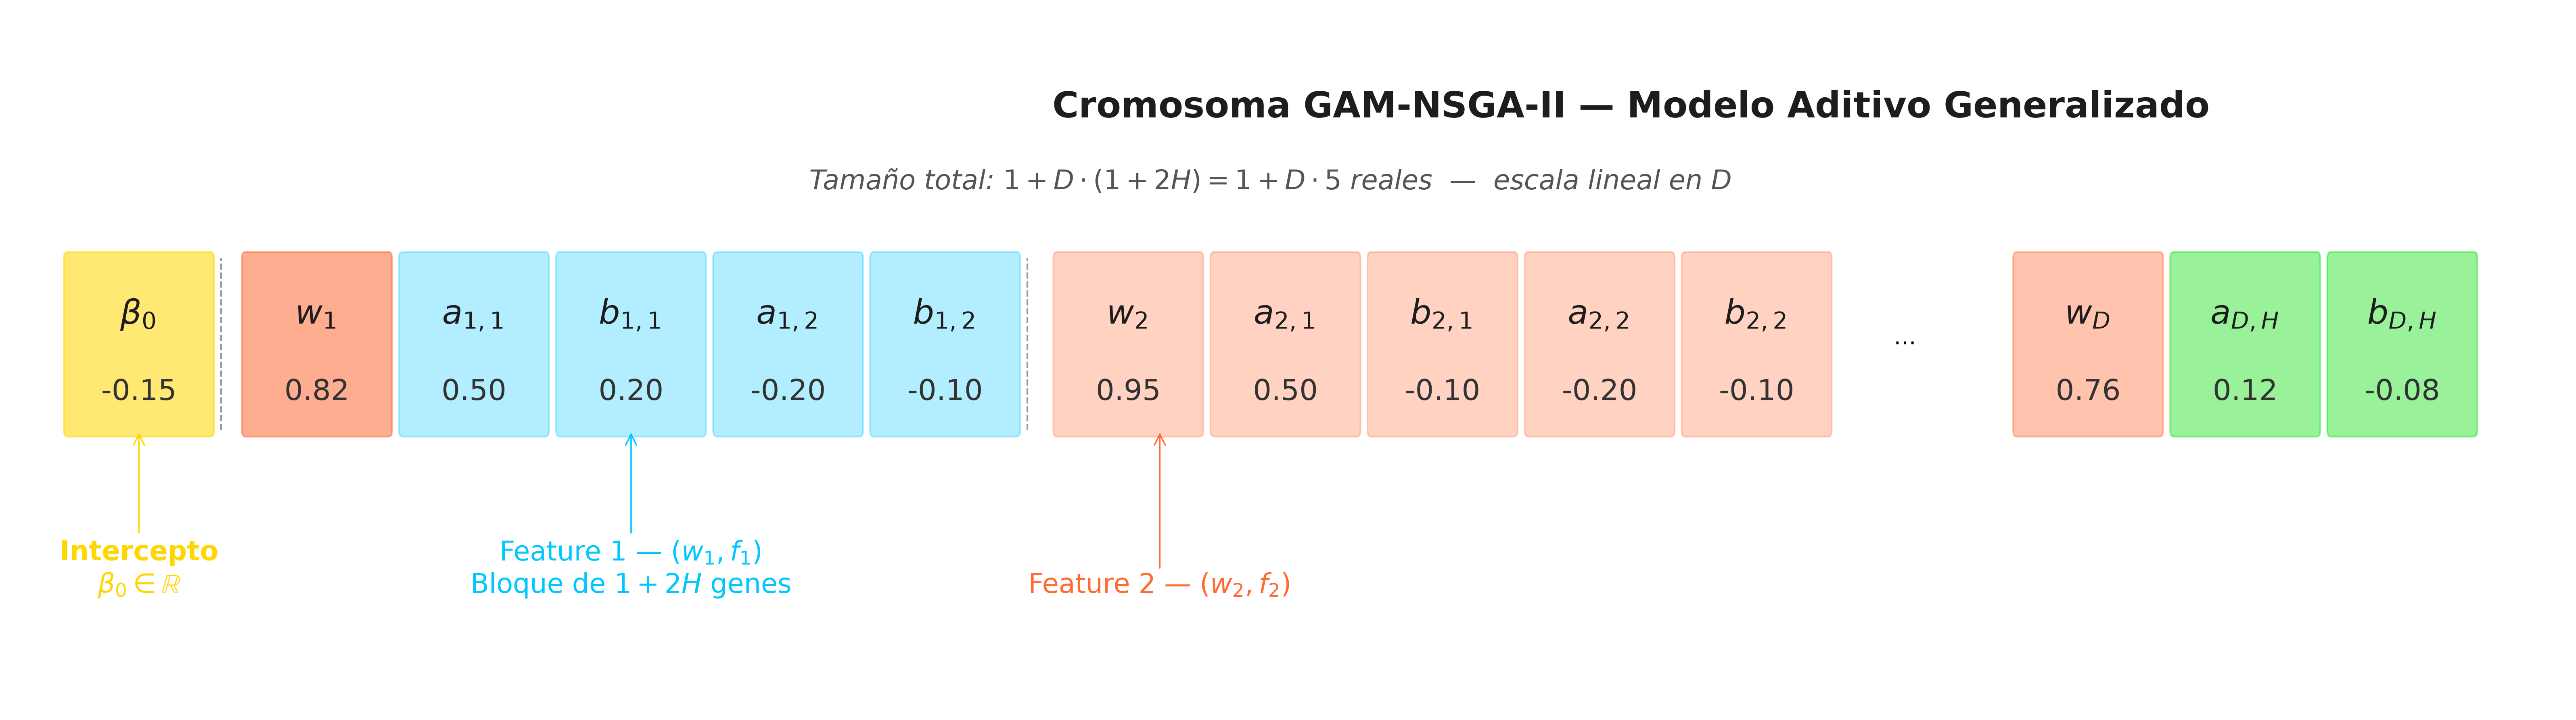
\includegraphics[width=0.85\textwidth]{../build/plot_gam_chromosome.png}
  \vspace{4pt}
  \begin{tcolorbox}[myex={¿Qué vemos?}]
    {\small El cromosoma GAM expande el AM a una \textbf{matriz de coeficientes} $D \times H$. Cada fila corresponde a un eje dimensional y cada columna a un armónico polinomial. Los pesos $\mathbf{w}$ (primera barra) son la Feature Importance directamente legible.}
  \end{tcolorbox}
\end{frame}

%% ── GEN 4: SHM ───────────────────────────────────────────────
\begin{frame}{Generación 4: Spherical Harmonic Manifold (SHM)}
  \textbf{Motivación:} AM/GAM tienen un solo eje de proyección — asimétrico para distribuciones complejas. ¿Cómo recuperar la expresividad de FM con la velocidad de AM?

  \begin{columns}[T]
    \begin{column}{0.55\textwidth}
      \textbf{Paso 1 — Base ortonormal 3D (Gram-Schmidt ponderado):}
      \[
        \{\mathbf{v}_1, \mathbf{v}_2, \mathbf{v}_3\} \subset \mathbb{R}^D, \quad \langle \mathbf{v}_i, \mathbf{v}_j \rangle_w = \delta_{ij}
      \]

      \textbf{Paso 2 — Proyección a $S^2$:}
      \[
        \theta = \arccos\!\left(\frac{\langle\mathbf{x}\!-\!\mathbf{c},\mathbf{v}_3\rangle_w}{\|\mathbf{x}\!-\!\mathbf{c}\|_w}\right),\quad \phi = \text{atan2}(p_2, p_1)
      \]

      \textbf{Paso 3 — Radio con Armónicos Esféricos Reales:}
      \[
        r^*(\theta,\phi) = \sum_{l=0}^{L}\sum_{m=-l}^{l} c_{l,m}\,Y_l^m(\theta,\phi)
      \]
    \end{column}
    \begin{column}{0.42\textwidth}
      \textbf{Los Armónicos Esféricos $Y_l^m$:}
      \[
        Y_l^m(\theta,\phi) = N_l^m\, P_l^{|m|}(\cos\theta)\cdot\begin{cases}\cos(m\phi)&m>0\\\!\!\sqrt{2}&m=0\\\sin|m|\phi&m<0\end{cases}
      \]
      donde $P_l^m$ son los \textbf{Polinomios Asociados de Legendre}.
      \vspace{4pt}
      \begin{block}{Complejidad}
        $\mathcal{O}(D + L^2)$ — sin búsqueda de $t^*$.
      \end{block}
      \begin{tcolorbox}[mywarn={Diferencia con AM}]
        {\small AM usa 1 eje $\Rightarrow$ 1 escalar.\\
        SHM usa 3 ejes $\Rightarrow$ deformación \textbf{volumétrica} en $S^2$.}
      \end{tcolorbox}
    \end{column}
  \end{columns}
\end{frame}

\begin{frame}{Armónicos Esféricos: Intuición Geométrica}
  \begin{columns}[T]
    \begin{column}{0.5\textwidth}
      Los $Y_l^m$ son las \textbf{funciones propias del Laplaciano en $S^2$}. Son la base ortonormal del espacio de funciones de la esfera, análogas a los senos y cosenos en la línea recta.

      \vspace{8pt}
      \textbf{¿Qué controla cada $(l, m)$?}
      \begin{itemize}
        \item $l=0$: radio constante (esfera perfecta)
        \item $l=1$: deformación dipolar (elongación en un eje)
        \item $l=2$: deformación cuadrupolar (forma de donut, silla de montar)
        \item $l \geq 3$: ondulaciones de alta frecuencia sobre la esfera
      \end{itemize}
    \end{column}
    \begin{column}{0.46\textwidth}
      \begin{tcolorbox}[myex={Ejemplo: Forma de patata}]
        {\small Queremos una frontera en 3D que tenga una protuberancia al Norte y una hendidura al Este.\\[4pt]
        $c_{0,0} = 1.0$ (radio base)\\
        $c_{1,0} = 0.3$ (elongar hacia el Norte)\\
        $c_{2,2} = -0.2$ (hundir hacia el Ecuador)\\[4pt]
        $r^*(\theta,\phi) = 1.0 \cdot Y_0^0 + 0.3 \cdot Y_1^0 - 0.2 \cdot Y_2^2$\\[4pt]
        El resultado: frontera con forma de \textbf{``patata deformada''}.}
      \end{tcolorbox}
    \end{column}
  \end{columns}
  \vspace{6pt}
  \centering
  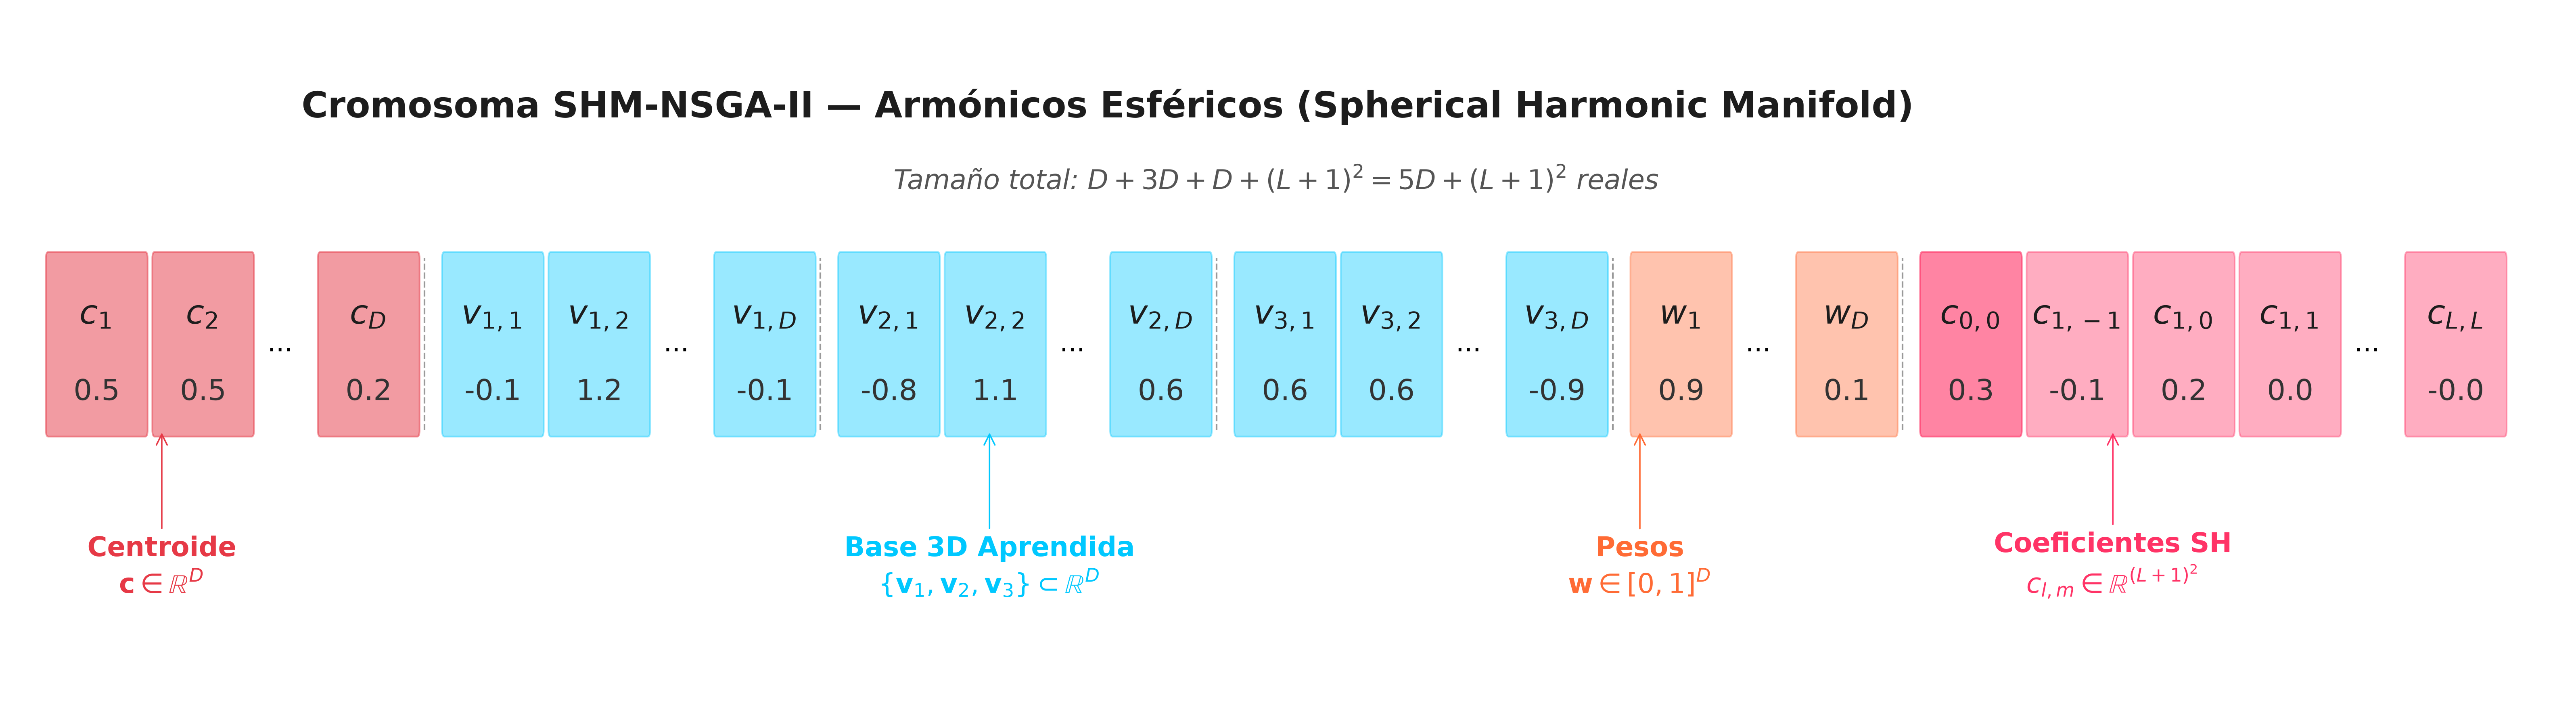
\includegraphics[width=0.85\textwidth]{../build/plot_shm_chromosome.png}
\end{frame}

%% ============================================================
\section{Estrategia de Clasificación: OvR e Inferencia}
%% ============================================================

\begin{frame}{One-vs-Rest (OvR) y la Regla de Inferencia}
  \begin{columns}[T]
    \begin{column}{0.5\textwidth}
      \begin{block}{Estrategia OvR}
        Para $K$ clases, se entrenan $K$ colectores independientes. El colector $M_k$ aprende a encapsular únicamente a la clase $k$, rechazando todas las demás.
      \end{block}
      \vspace{6pt}
      \textbf{Regla de asignación final:}
      \[
        k^* = \arg\min_k \bigl(D_S(\mathbf{x}, M_k)\bigr)
      \]
      El punto pertenece al colector que lo ``atrapa'' con mayor profundidad (distancia con signo más negativa).
    \end{column}
    \begin{column}{0.47\textwidth}
      \begin{tcolorbox}[myex={Diagnóstico médico 3 clases}]
        {\small Clases: [Sano, Neumonía, COVID-19].\\[6pt]
        Para un Paciente X:\\
        $D_S(M_{\text{Sano}}) = +4.2$ \textcolor{accent2}{(fuera)}\\
        $D_S(M_{\text{Neumonia}}) = -0.5$ \textcolor{accent3}{(dentro)}\\
        $D_S(M_{\text{COVID}}) = -3.8$ \textcolor{accent3}{(muy dentro)}\\[6pt]
        $\arg\min = -3.8 \Rightarrow$ \textbf{COVID-19}\\[4pt]
        La profundidad de $-3.8$ da \textbf{certidumbre analítica}.}
      \end{tcolorbox}
    \end{column}
  \end{columns}
\end{frame}

%% ============================================================
\section{Motores de Optimización}
%% ============================================================

\begin{frame}{Motor 1: NSGA-II (Optimización Evolutiva Multi-Objetivo)}
  \begin{columns}[T]
    \begin{column}{0.55\textwidth}
      Minimizamos \textbf{dos objetivos conflictivos} simultáneamente:
      \[
        \mathbf{O} = [O_1, O_2]^T
      \]
      \begin{itemize}
        \item \textbf{$O_1$ — Error empírico:}
        \[
          O_1 = \frac{1}{N}\sum_i \mathbb{I}[y_i \neq \operatorname{sign}(-D_S)]
        \]
        \item \textbf{$O_2$ — Complejidad (Navaja de Ockham):}\\
        Longitud de la curva + número de armónicos $H$ + regularización $L_1$ sobre $\mathbf{w}$.
      \end{itemize}
      \vspace{6pt}
      NSGA-II mantiene una \textbf{población} de soluciones no-dominadas formando el \textbf{Frente de Pareto}.
    \end{column}
    \begin{column}{0.42\textwidth}
      \begin{tcolorbox}[myex={¿Por qué dos objetivos?}]
        {\small Un colector con $O_1=0$ (cero error) y $O_2=\infty$ es un caos de tentáculos que memoriza ruido — \textbf{overfitting}.\\[4pt]
        Un colector con $O_2=0$ (mínima complejidad, un círculo) generalmente tiene $O_1 > 0$ — \textbf{underfitting}.\\[4pt]
        NSGA-II nos entrega \textbf{todo el espectro} de soluciones de equilibrio.}
      \end{tcolorbox}
      \begin{alertblock}{Pareto $\neq$ óptimo único}
        El usuario elige el punto del frente que mejor se adapta a sus restricciones.
      \end{alertblock}
    \end{column}
  \end{columns}
\end{frame}

\begin{frame}{Motor 2: MGDA — El Salto Diferencial}
  \begin{columns}[T]
    \begin{column}{0.55\textwidth}
      \textbf{Condición para usar MGDA:} Los kernels AM y GAM son diferenciables:
      \[
        \nabla_\theta O_1 \text{ y } \nabla_\theta O_2 \text{ existen analíticamente.}
      \]

      La dirección de descenso conjunta óptima:
      \[
        \mathbf{d} = -\bigl(\alpha\,\nabla O_1 + (1-\alpha)\,\nabla O_2\bigr)
      \]
      donde $\alpha \in [0,1]$ es el \textbf{peso de Pareto} que determina el punto del frente.

      \vspace{6pt}
      \textbf{Actualización de parámetros:}
      \[
        \theta_{t+1} = \theta_t - \eta\,\mathbf{d}
      \]
      Con optimizadores modernos: \textbf{Adam}, \textbf{Focal Loss}.
    \end{column}
    \begin{column}{0.42\textwidth}
      \begin{tcolorbox}[myex={El árbitro geométrico}]
        {\small En la iteración 100, los gradientes \textbf{conflictúan}:
        \begin{itemize}
          \item $\nabla O_1$: ``Ir al \textbf{Norte} para abarcar un dato perdido''
          \item $\nabla O_2$: ``Ir al \textbf{Sur}, la curva se vuelve inestable''
        \end{itemize}
        MGDA calcula el ángulo de conflicto y resuelve: ir al \textbf{Oeste} — reduce el error sin destruir la topología.}
      \end{tcolorbox}
      \begin{alertblock}{Aceleración}
        De decenas de segundos (NSGA-II) a \textbf{fracciones de segundo} (MGDA). Viable para \textbf{Edge AI}.
      \end{alertblock}
    \end{column}
  \end{columns}
\end{frame}

\begin{frame}{El Frente de Pareto: Visualización}
  \centering
  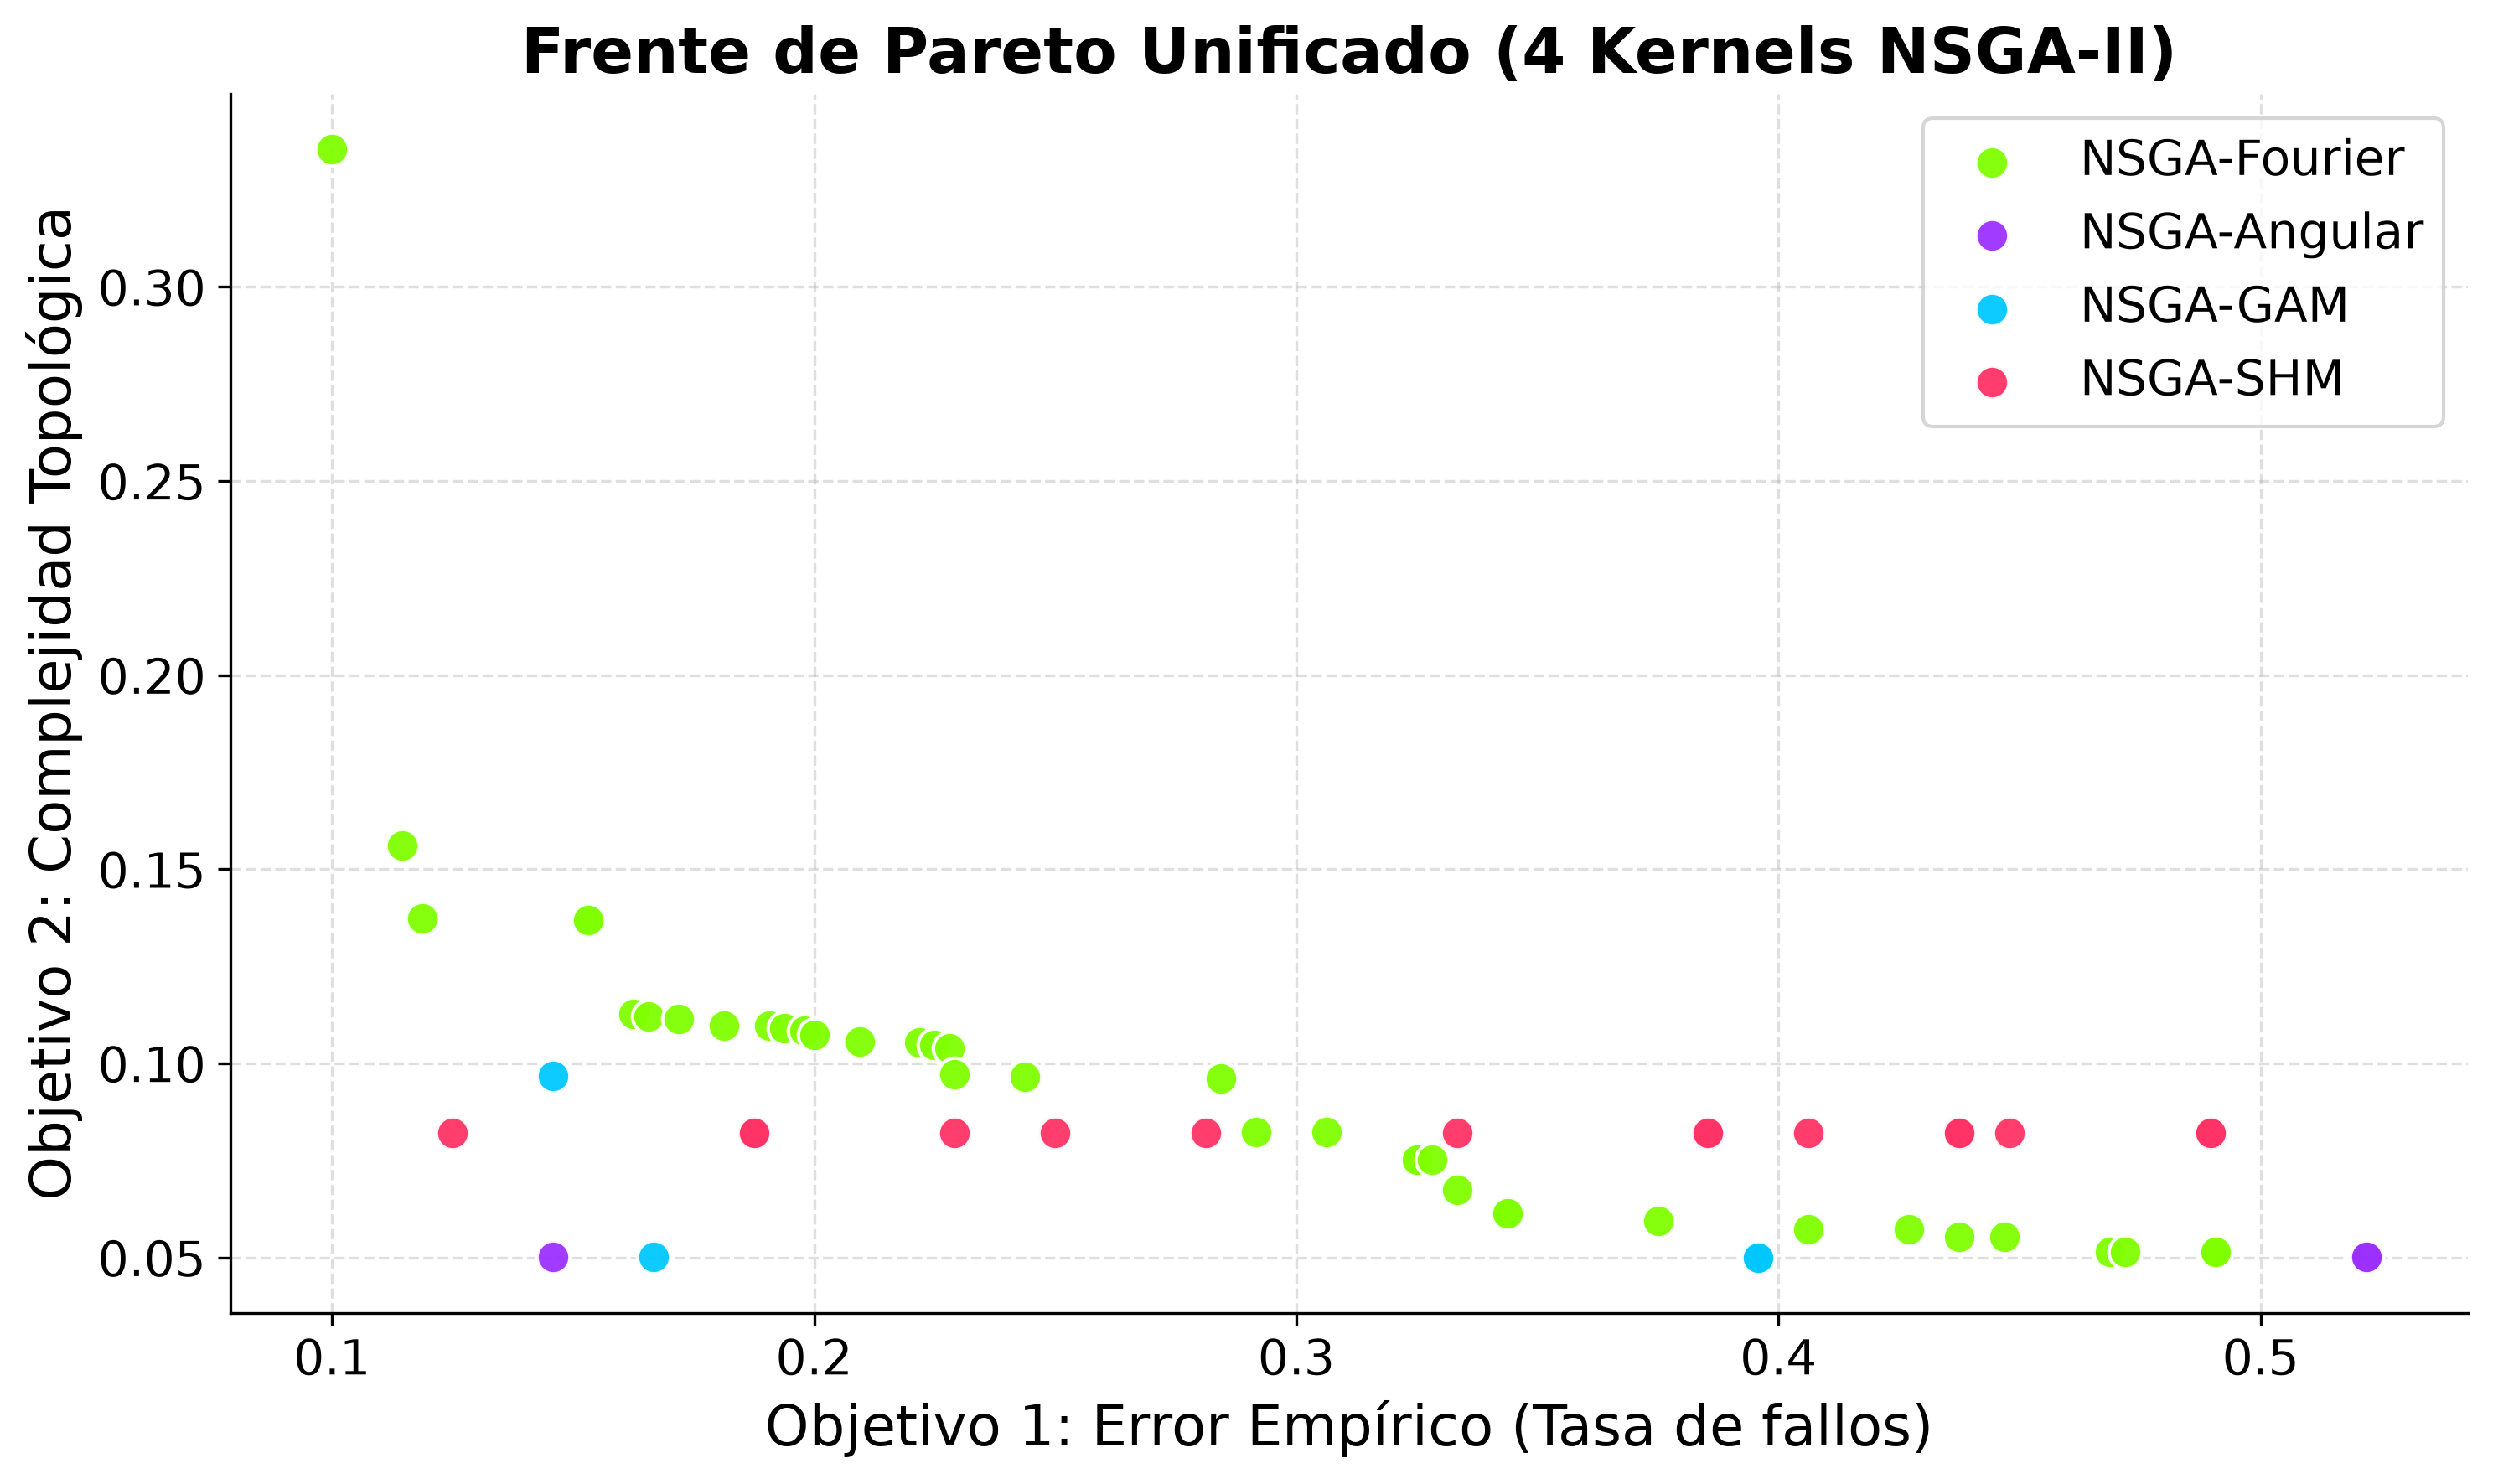
\includegraphics[width=0.78\textwidth]{../build/plot_pareto_3kernels.png}
  \vspace{4pt}
  \begin{tcolorbox}[myex={Interpretación}]
    {\small Cada punto en el gráfico es una \textbf{solución válida} no-dominada. Las soluciones a la izquierda-arriba tienen \textbf{baja complejidad, mayor error}. Las de la derecha-abajo tienen \textbf{alta complejidad, menor error}. Un ingeniero elige el punto de equilibrio óptimo para su aplicación.}
  \end{tcolorbox}
\end{frame}

\begin{frame}{Comparación del Frente de Pareto: MGDA vs NSGA-II}
  \centering
  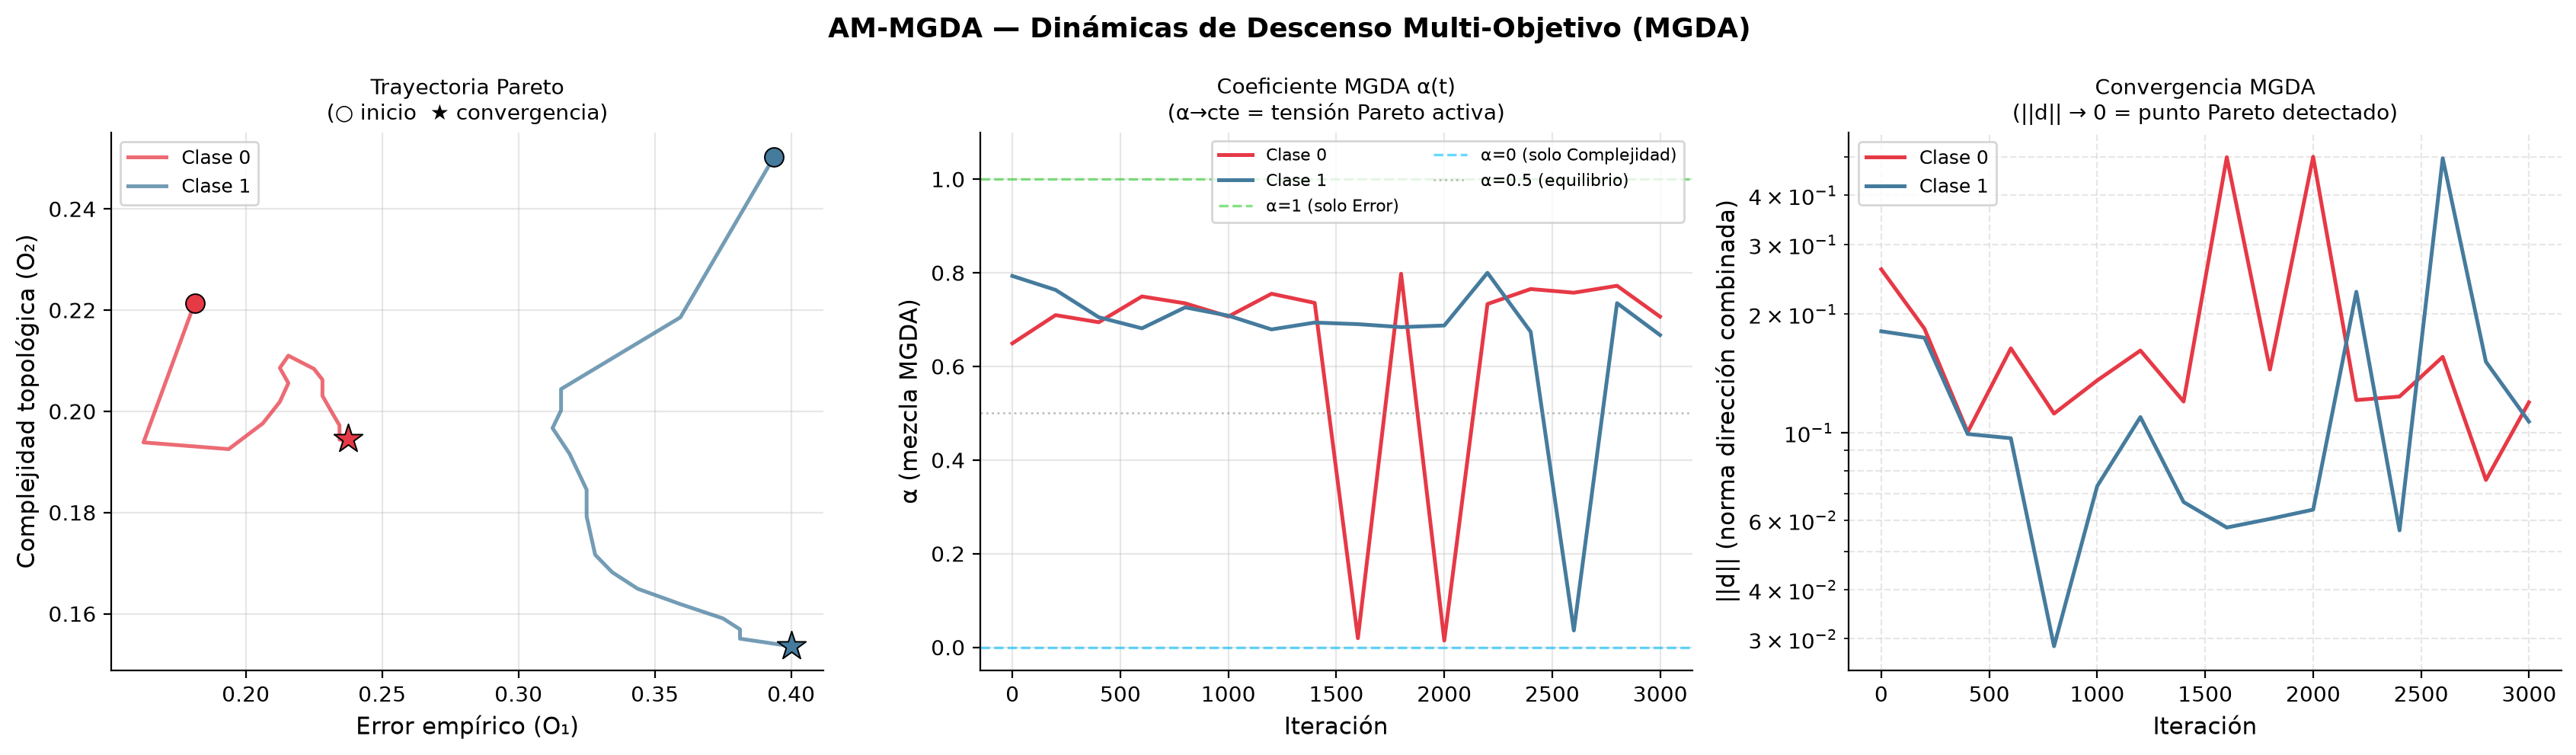
\includegraphics[width=0.82\textwidth]{../build/mgda_plot.png}
  \vspace{4pt}
  \begin{columns}[T]
    \begin{column}{0.48\textwidth}
      \textbf{NSGA-II}: muchas generaciones para converger al frente — cada iteración evalúa cientos de candidatos.
    \end{column}
    \begin{column}{0.48\textwidth}
      \textbf{MGDA}: sigue el gradiente hacia el frente en \textbf{pasos exactos} — convergencia orders of magnitude más rápida.
    \end{column}
  \end{columns}
\end{frame}

%% ============================================================
\section{Análisis Visual de las Variedades}
%% ============================================================

\begin{frame}{Colectores en Acción: Datasets 2D}
  \centering
  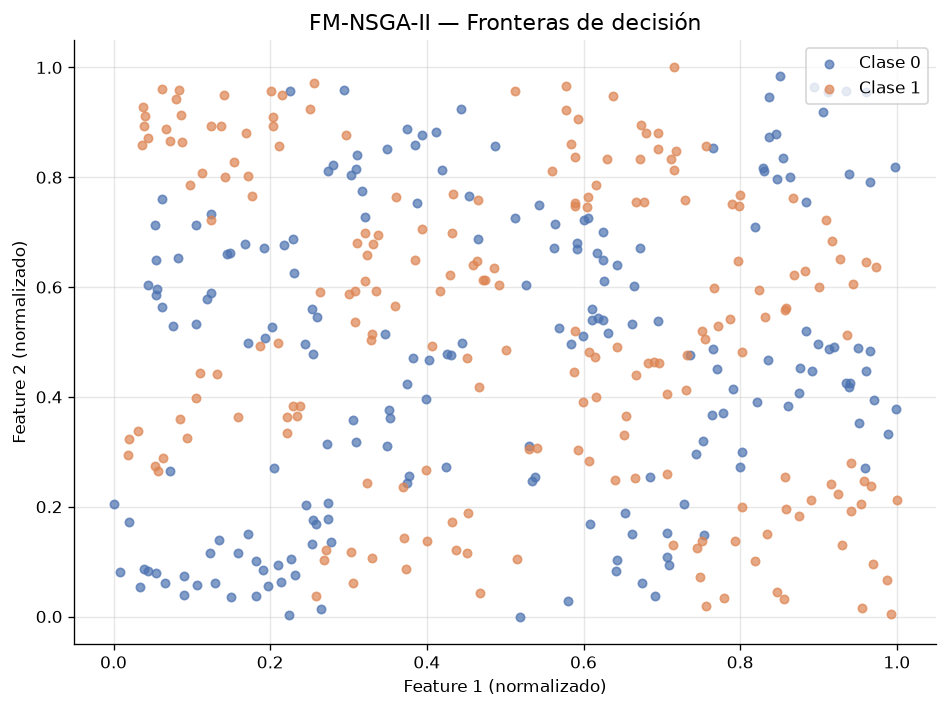
\includegraphics[width=0.90\textwidth]{../build/plot_dataset.png}
  \vspace{4pt}
  \begin{tcolorbox}[myex={¿Qué vemos?}]
    {\small Los colectores parametrizados se adaptan a la topología nativa de los datos. En \textit{Two Moons}, la curva literalmente ``abraza'' la forma de luna. En \textit{Circles}, genera dos fronteras concéntricas anidadas. La ecuación matemática de cada frontera es \textbf{completamente extractable e imprimible}.}
  \end{tcolorbox}
\end{frame}

%% ============================================================
\section{Resultados Experimentales}
%% ============================================================

\begin{frame}{Benchmark Global: Accuracy}
  \centering
  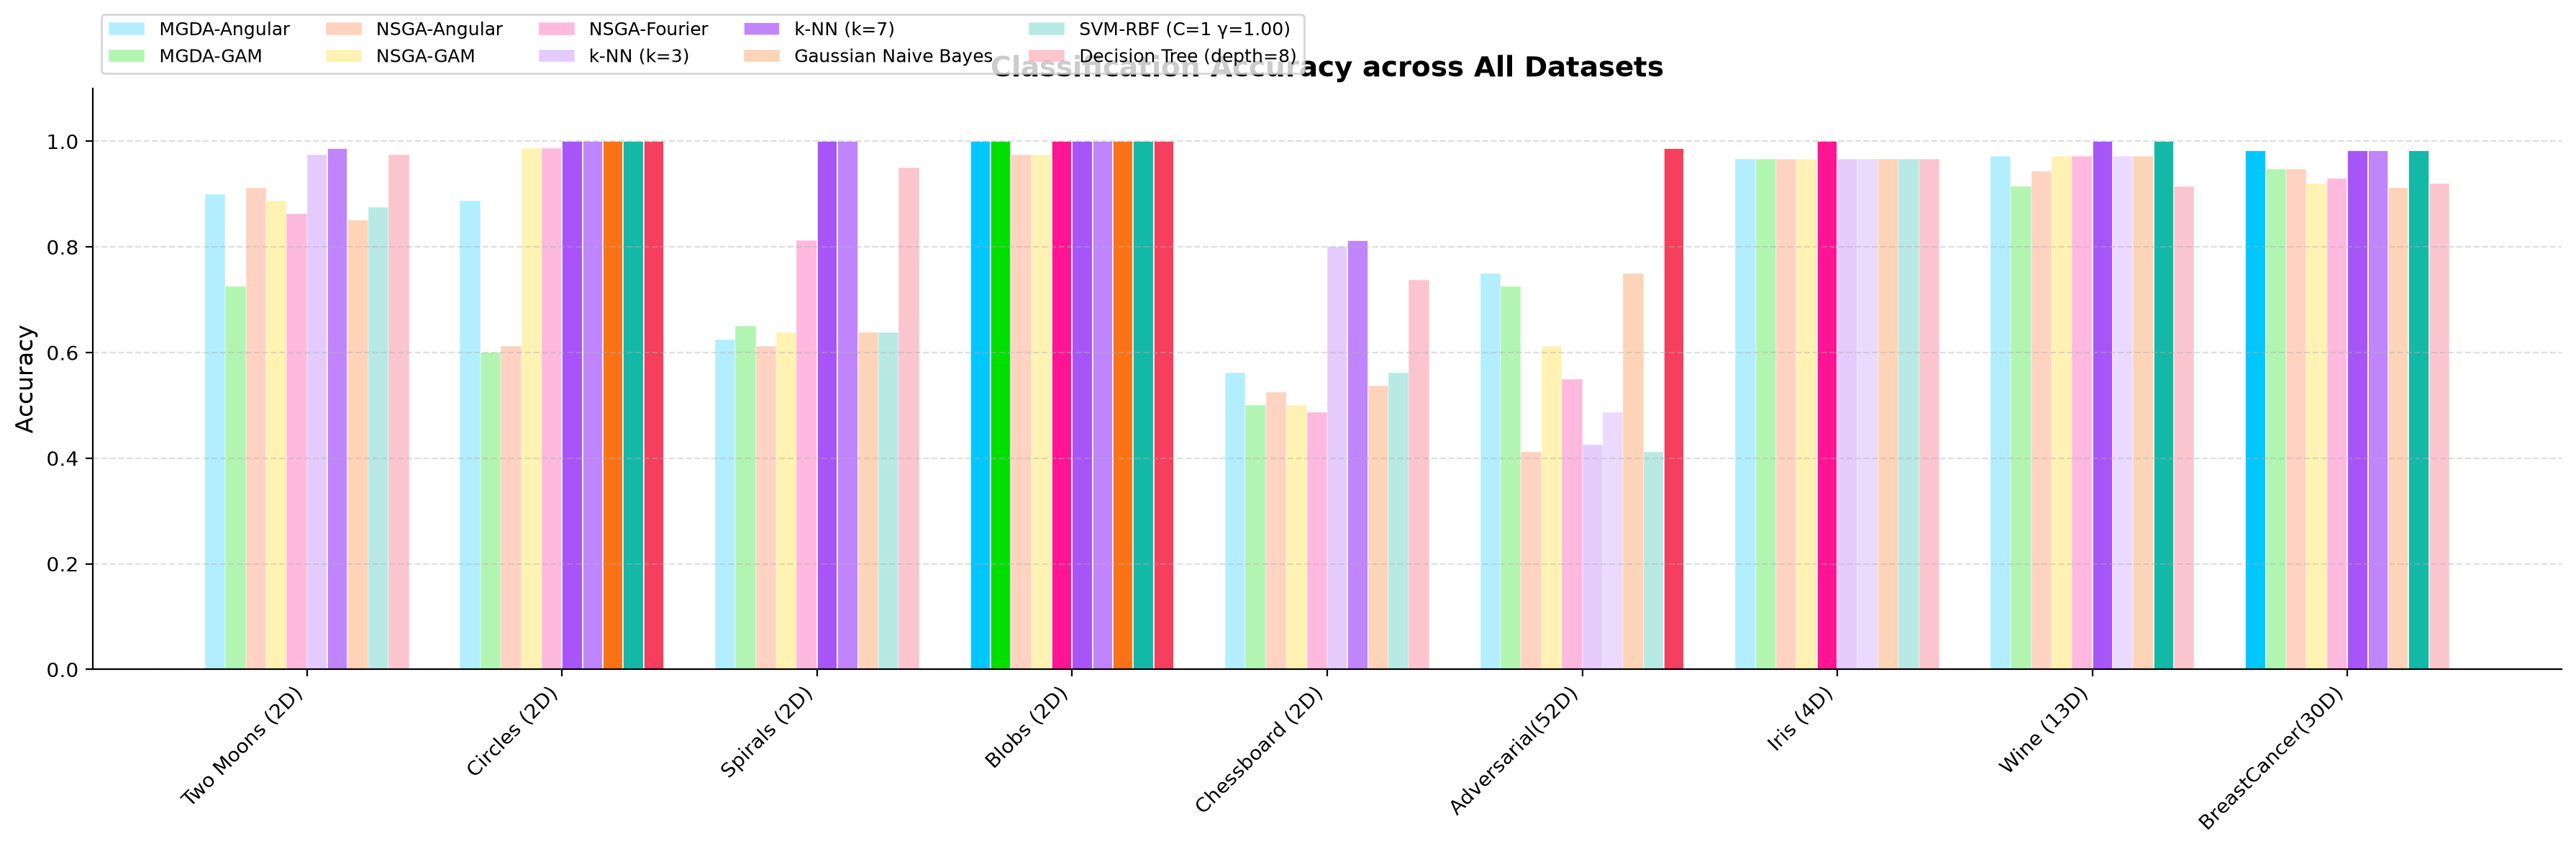
\includegraphics[width=\textwidth]{../build/benchmark_acc.png}
  \vspace{4pt}
  {\small
  \begin{itemize}
    \item La familia topológica propuesta \textbf{iguala o supera} a los modelos clásicos en la mayoría de datasets.
    \item MGDA \textbf{conserva} la accuracy descubierta por NSGA-II, sin sacrificarla por la velocidad.
    \item El modelo se desploma en \textit{Adversarial Noise (52D)} — la \textbf{maldición de dimensionalidad} afecta a todos los métodos basados en distancia.
  \end{itemize}}
\end{frame}

\begin{frame}{Asimetría Computacional: Tiempos de Entrenamiento}
  \centering
  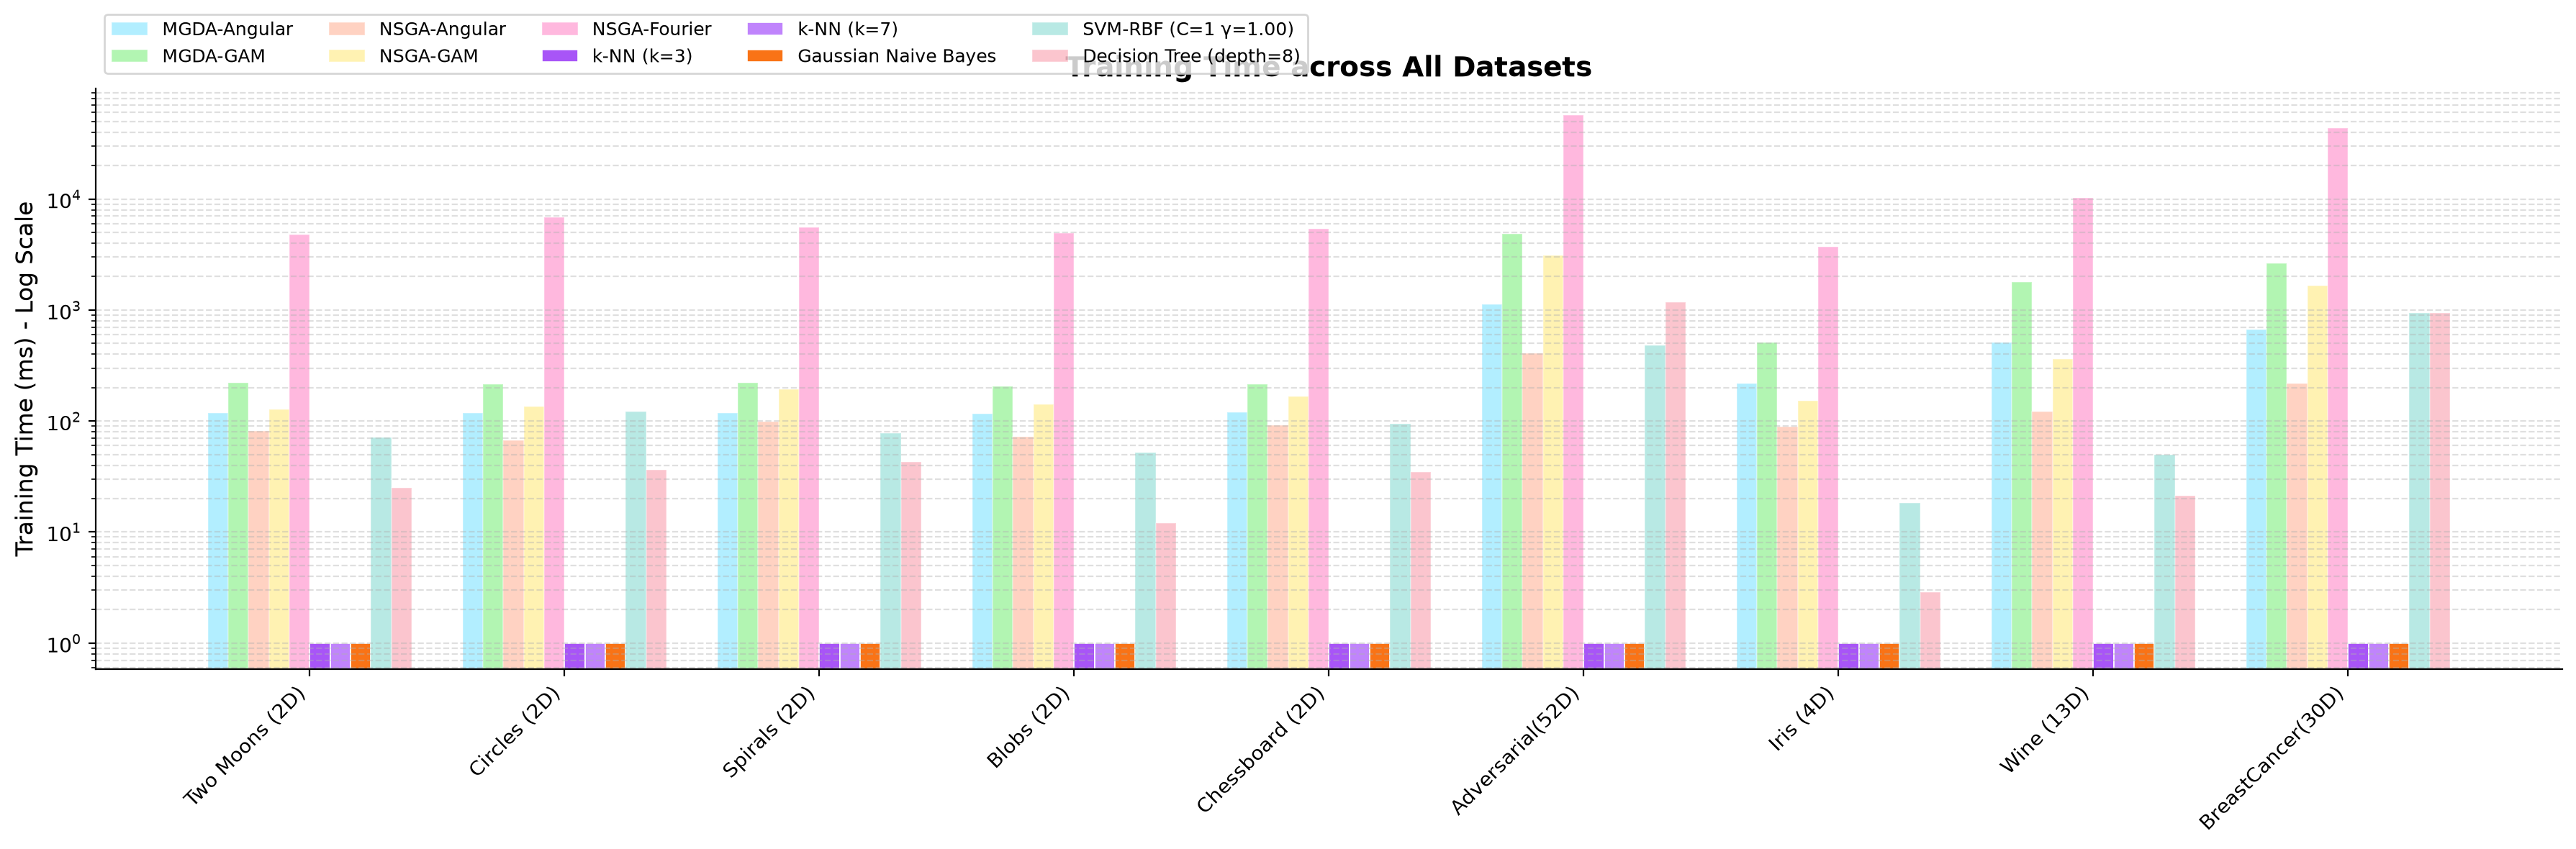
\includegraphics[width=\textwidth]{../build/benchmark_time.png}
  \vspace{4pt}
  {\small
  \begin{itemize}
    \item \textbf{FM-NSGA-II}: miles de ms en \textit{Two Moons} — la trigonometría es el cuello de botella.
    \item \textbf{AM-NSGA-II}: ya mucho más rápido por Chebyshev sin $t^*$.
    \item \textbf{MGDA-GAM}: colapsa a fracciones de segundo — \textbf{$>100\times$ más rápido}.
    \item En \textit{Breast Cancer (30D)}: la familia NSGA colapsa; MGDA lo resuelve al instante.
  \end{itemize}}
\end{frame}

\begin{frame}{Validación Estadística: Test de Wilcoxon}
  \begin{columns}[T]
    \begin{column}{0.55\textwidth}
      \textbf{¿Qué es el test de Wilcoxon?}\\
      Prueba no paramétrica (Demšar, 2006) para comparar dos algoritmos sobre múltiples datasets.\\[6pt]
      \textbf{Hipótesis:} ¿La diferencia entre modelo A y B es sistemática (real) o al azar?\\[6pt]
      \textbf{Criterio:} $p < 0.05 \Rightarrow$ diferencia estadísticamente significativa.
    \end{column}
    \begin{column}{0.42\textwidth}
      \begin{tcolorbox}[myex={Nuestros resultados}]
        {\footnotesize
        \textbf{Accuracy}: $p > 0.05$ en todos los cruces\\
        $\Rightarrow$ \textcolor{accent3}{No hay diferencia significativa}\\
        $\Rightarrow$ Nuestra White-Box no sacrifica precisión.\\[6pt]
        \textbf{Tiempo (ms)}: $p = 0.0039$ en todos\\
        $\Rightarrow$ \textcolor{accent2}{Diferencia contundente}\\
        $\Rightarrow$ La aceleración es estadísticamente irrefutable.}
      \end{tcolorbox}
    \end{column}
  \end{columns}
  \vspace{8pt}
  \begin{alertblock}{Síntesis estadística}
    Los colectores topológicos son \textbf{irrefutablemente más rápidos} que la generación anterior, y estadísticamente \textbf{equivalentes} en precisión a las cajas negras del estado del arte.
  \end{alertblock}
\end{frame}

%% ============================================================
\section{Interpretabilidad Analítica: Feature Importance}
%% ============================================================

\begin{frame}{White-Box: Feature Importance nativa del GAM}
  \begin{columns}[T]
    \begin{column}{0.5\textwidth}
      El vector $\mathbf{w} = [w_1, \ldots, w_D]$ del cromosoma GAM es el \textbf{único y exacto} certificado de importancia de features.

      \vspace{8pt}
      \textbf{Mecanismo matemático:}
      \[
        R(\mathbf{x}) = a_0 + \sum_{d=1}^{D} \underbrace{w_d}_{\text{importancia}} \cdot \phi_d(\hat{x}_d)
      \]
      Si el optimizador fuerza $w_d \to 0$, el eje $d$ queda \textbf{matemáticamente anulado} en la sumatoria.

      \vspace{8pt}
      No se requiere:
      \begin{itemize}
        \item LIME (aproximaciones locales post-hoc)
        \item SHAP (valores de Shapley computacionalmente caros)
        \item Ninguna aproximación — es \textbf{exacto}.
      \end{itemize}
    \end{column}
    \begin{column}{0.47\textwidth}
      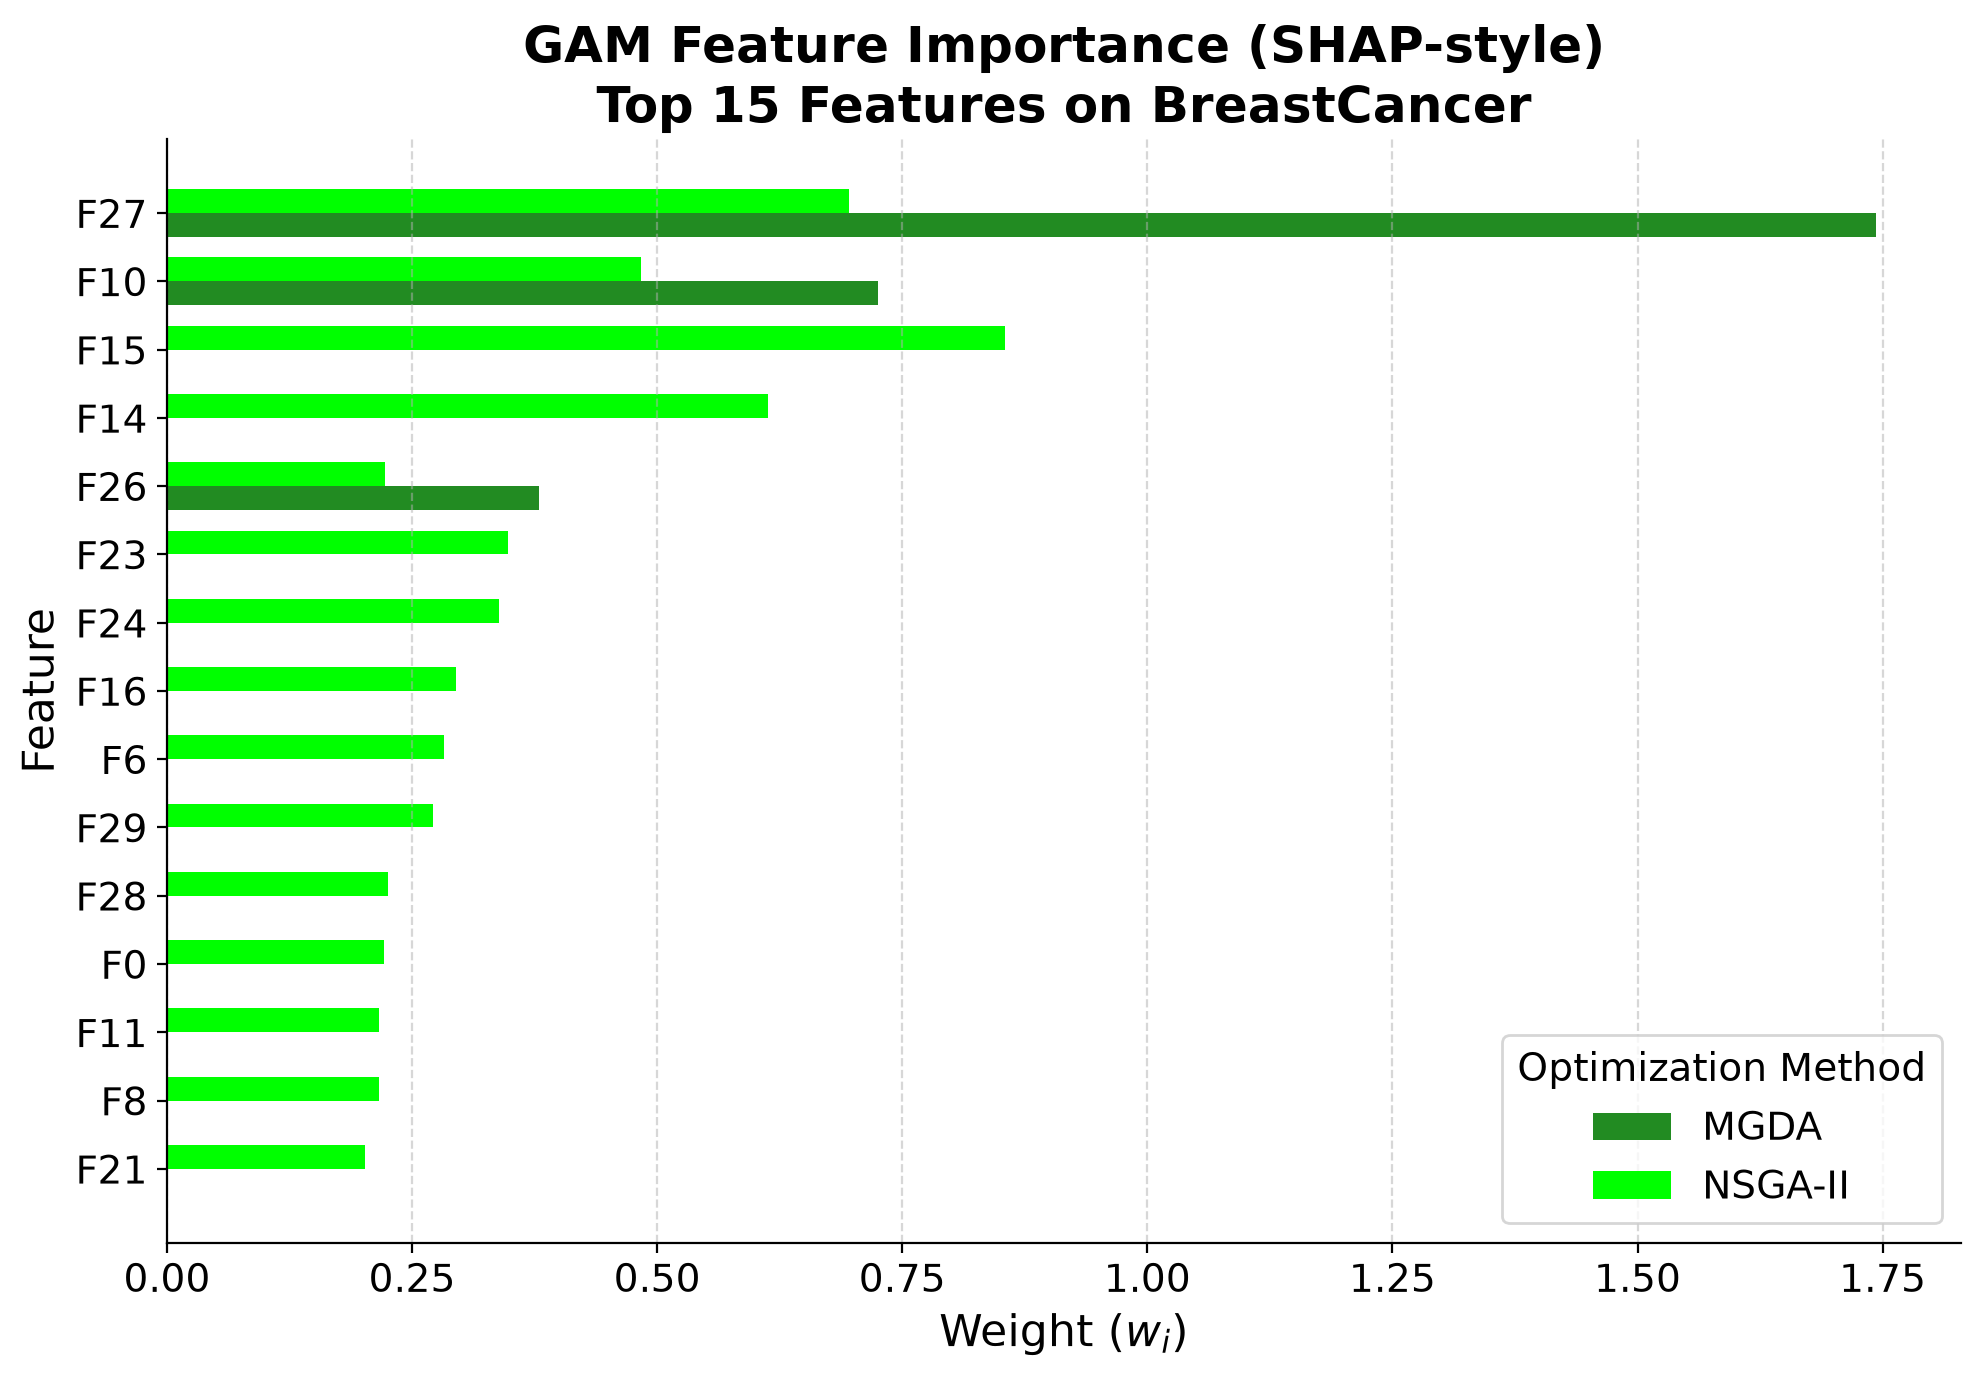
\includegraphics[width=\textwidth]{../build/gam_importance.png}
      \vspace{4pt}
      {\small \textbf{Breast Cancer (30D)}: el modelo suprimió $>60\%$ de las dimensiones de ruido, concentrando la decisión en los factores morfológicos diagnósticos reales.}
    \end{column}
  \end{columns}
\end{frame}

%% ============================================================
\section{El Límite y Trabajo Futuro}
%% ============================================================

\begin{frame}{La Maldición de Dimensionalidad}
  \begin{columns}[T]
    \begin{column}{0.55\textwidth}
      \textbf{Dataset: Adversarial Noise (52D)}\\
      Dos círculos en 2D ofuscados por \textbf{50 dimensiones de ruido puro}.
      \vspace{6pt}

      \textbf{¿Qué ocurre?}
      \begin{itemize}
        \item En 52D, las distancias euclidianas se \textbf{homogenizan} — todos los puntos están a distancias similares (concentración de medidas).
        \item Los pesos $\mathbf{w}$ del NSGA-II o los gradientes de MGDA son abrumados por el volumen del hipercubo.
        \item \textbf{Resultado:} $\approx 50\%$ Accuracy — equivalente al azar.
      \end{itemize}

      \vspace{6pt}
      \textbf{Excepciones:}\\
      Solo los \textbf{Árboles de Decisión} salvaron la señal — su bifurcación ortogonal actúa como \textbf{descarte topológico exacto} de hiperplanos.
    \end{column}
    \begin{column}{0.42\textwidth}
      \begin{tcolorbox}[mywarn={Límite fundamental}]
        {\small Los colectores paramétricos basan su inferencia en \textbf{distancias radiales}. En alta dimensión con ruido dominante, la señal útil se ahoga en el denominador de la norma euclidiana.}
      \end{tcolorbox}
      \vspace{8pt}
      \begin{block}{Trabajo Futuro}
        \begin{itemize}
          \item Combinar GAM con \textbf{selección de features adaptativa}.
          \item \textbf{MGDA para SHM}: requiere el jacobiano de la proyección Gram-Schmidt y la evaluación de $Y_l^m$.
          \item Extensión a clasificación \textbf{multi-label}.
        \end{itemize}
      \end{block}
    \end{column}
  \end{columns}
\end{frame}

%% ============================================================
\section{Síntesis y Conclusiones}
%% ============================================================

\begin{frame}{Tabla Comparativa de Generaciones}
  \centering
  {\small
  \begin{tabular}{lcccc}
    \toprule
    \textbf{Modelo} & \textbf{Complejidad} & \textbf{Auditable} & \textbf{Optimizador} & \textbf{Velocidad relativa}\\
    \midrule
    FM-NSGA-II  & $O(D \cdot H)$ + búsqueda $t^*$ & Parcial & NSGA-II & 1$\times$ (base) \\
    AM-NSGA-II  & $O(D + H)$                       & Media   & NSGA-II & $\sim 5\times$ \\
    GAM-NSGA-II & $O(D \cdot H)$                   & \textcolor{accent3}{\textbf{Total}} & NSGA-II & $\sim 5\times$ \\
    SHM-NSGA-II & $O(D + L^2)$                     & Media   & NSGA-II & $\sim 4\times$ \\
    AM-MGDA     & $O(D + H)$                        & Media   & \textcolor{accent3}{\textbf{MGDA}}   & $\mathbf{>100\times}$ \\
    GAM-MGDA    & $O(D \cdot H)$                   & \textcolor{accent3}{\textbf{Total}} & \textcolor{accent3}{\textbf{MGDA}}   & $\mathbf{>100\times}$ \\
    \bottomrule
  \end{tabular}}
  \vspace{8pt}
  \begin{columns}
    \begin{column}{0.48\textwidth}
      \textbf{GAM-MGDA} es el punto óptimo del espacio de diseño:\\
      máxima auditabilidad + máxima velocidad.
    \end{column}
    \begin{column}{0.48\textwidth}
      \textbf{SHM-NSGA-II} es la frontera de expresividad:\\
      recupera la morfología volumétrica de FM con inferencia polinomial.
    \end{column}
  \end{columns}
\end{frame}

\begin{frame}{Conclusiones}
  \begin{enumerate}
    \item \highlight{Cajas Blancas Geométricas:}\\
    Las variedades paramétricas resuelven topologías en herradura, luna y espiral \textbf{sin sacrificar la ecuación matemática gobernante}.
    \vspace{6pt}

    \item \highlight{Trigonometría precisa pero costosa:}\\
    FM brinda expresividad extrema pero es \textbf{computacionalmente prohibitivo} para Big Data y Edge AI.
    \vspace{6pt}

    \item \highlight{Aislamiento $\Rightarrow$ Auditoría:}\\
    Transicionar de Fourier acoplado (FM) a polinomios independientes por eje (GAM) entrega un vector $\mathbf{w}$ que indica \textbf{exactamente qué variables} tomaron la decisión, sin aproximaciones post-hoc.
    \vspace{6pt}

    \item \highlight{El Salto Diferencial ($>100\times$):}\\
    MGDA cristaliza la tecnología paramétrica como \textbf{alternativa viable para Edge AI}, destruyendo los tiempos del motor evolutivo sin perder precisión topológica.
    \vspace{6pt}

    \item \highlight{Validación estadística irrefutable:}\\
    El test de Wilcoxon ($p = 0.0039$ en tiempos) certifica con rigor científico que la aceleración es \textbf{sistemática y real}, no un artefacto de un dataset particular.
  \end{enumerate}
\end{frame}

%% ── CIERRE ───────────────────────────────────────────────────
{
\setbeamercolor{background canvas}{bg=primary}
\begin{frame}[plain]
  \centering
  \vspace{2cm}
  {\Huge\bfseries\textcolor{accent}{¿Preguntas?}}\\[20pt]
  \rule{6cm}{0.4pt}\\[12pt]
  {\large\textcolor{white}{Hugo Campos Castro}}\\[6pt]
  {\small\textcolor{white!60}{Clasificación Topológica via Variedades Paramétricas\\FM $\to$ AM $\to$ GAM $\to$ SHM $\|$ NSGA-II $\to$ MGDA}}\\[20pt]
  {\small\textcolor{accent!70}{Repositorio: github.com/uwo-o/FM-NSGA-II}}
\end{frame}
}

\begin{thebibliography}{9}
\bibitem{deb2002fast}
K.\ Deb et al., ``A fast and elitist multiobjective genetic algorithm: NSGA-II,''
\textit{IEEE Trans.\ Evol.\ Comput.}, vol.\ 6, no.\ 2, pp.\ 182--197, 2002.
\bibitem{desmar2006}
J.\ Dem\v{s}ar, ``Statistical comparisons of classifiers over multiple data sets,''
\textit{Journal of Machine Learning Research}, vol.\ 7, pp.\ 1--30, 2006.
\bibitem{siarry2016}
P.\ Siarry (Ed.), \textit{Metaheuristics}. Springer, 2016.
\end{thebibliography}

\end{document}
